\documentclass[conference]{IEEEtran}
\usepackage{graphicx}

\begin{document}

\title{Projeto Calculadora de Radiologia: Aprimoramento de Precisão de Cálculo}
\author{\IEEEauthorblockN{Roger da Palma, Guilherme Painko, Meani Freitas}
\IEEEauthorblockA{Universidade Franciscana\\
Endereço: R. dos Andradas, 1614 - Centro, Santa Maria - RS, 97010-030\\
Email: {rogerdapalma@gmail.com, gui.painko2393@gmail.com, meani.sf@gmail.com }}}

\maketitle

\begin{abstract}
Este artigo apresenta o desenvolvimento e a implementação de uma Calculadora de Radiologia, uma ferramenta inovadora projetada para aprimorar a precisão dos cálculos em procedimentos radiológicos. A aplicação visa auxiliar profissionais da área médica, oferecendo uma interface intuitiva e configurações dinâmicas para parâmetros cruciais, como K.V (Kilovoltagem), M.S (Tempo de Exposição) e M.A (Corrente do Tubo). Contextualizado com cunho extensionista.
\end{abstract}

\section{Introdução}
A radiologia desempenha um papel fundamental no diagnóstico médico, fornecendo imagens internas do corpo para avaliação clínica. A qualidade dessas imagens depende diretamente da precisão dos parâmetros utilizados durante o procedimento radiológico. A Calculadora de Radiologia surge como uma resposta a essa necessidade, visando simplificar e aprimorar o processo de configuração desses parâmetros.

\section{Objetivos do Projeto}
O principal objetivo deste projeto é desenvolver uma ferramenta acessível e eficiente que permita aos profissionais de radiologia realizar cálculos precisos para diferentes procedimentos de imagem. Os objetivos específicos incluem:

\begin{itemize}
  \item Proporcionar uma interface amigável para a entrada de dados, como região do corpo, tipo de projeção e espessura.
  \item Permitir a configuração dinâmica de parâmetros essenciais, como K.V, M.S e M.A.
  \item Aprimorar a precisão dos cálculos, considerando a região específica do corpo e outros fatores relevantes.
\end{itemize}

\section{Metodologia de Desenvolvimento}
A criação da Calculadora de Radiologia foi conduzida por meio da aplicação de tecnologias de ponta, evidenciando a utilização de HTML, CSS e JavaScript para a construção da interface do usuário. O design responsivo foi efetivado pela integração do framework Bulma, proporcionando uma experiência visual moderna e adaptativa.

A lógica de negócios e o controle de fluxo de dados foram implementados utilizando o framework Spring Boot, que facilita o desenvolvimento de aplicativos Java robustos e escaláveis. O Spring Boot adota a arquitetura Modelo-Visão-Controlador (MVC), que organiza o código de forma modular, melhorando a manutenibilidade e a escalabilidade do projeto.

A implementação do banco de dados MySQL desempenhou um papel fundamental na estruturação e armazenamento eficiente de dados. As funcionalidades específicas dessa tecnologia foram incorporadas para garantir a persistência e integridade das informações, ampliando a robustez e utilidade da Calculadora de Radiologia.

\section{Tecnologias Utilizadas}
O desenvolvimento da Calculadora de Radiologia utilizou diversas tecnologias essenciais, incluindo:

\begin{itemize}
  \item \textbf{Spring Data JPA:} Facilitou o acesso a dados relacionais e a persistência de dados.
  \item \textbf{MVC (Model-View-Controller):} Adotado pelo Spring Boot, organizou o código de forma modular.
  \item \textbf{Thymeleaf:} Utilizado para renderizar templates HTML no lado do servidor, facilitando a integração com o Spring Boot.
  \item \textbf{CSS (Bulma):} O framework Bulma proporcionou estilos responsivos e modernos para a interface do usuário.
\end{itemize}

\section{Funcionalidades Implementadas}
O projeto incorporou diversas funcionalidades para aprimorar a experiência do usuário e a eficácia da Calculadora de Radiologia, incluindo:

\begin{itemize}
\item \textbf{Autenticação de Usuários:} Implementação de uma tela de login que possibilita o cadastro e acesso seguro para os usuários. Esta funcionalidade visa proporcionar uma experiência personalizada e segura.
\item \textbf{Seleção de Região e Projeção:} Permite ao usuário escolher a região do corpo em exame e o tipo de projeção desejado (frontal ou lateral).
\item \textbf{Entrada de Espessura:} Fornece um campo dedicado para inserção da densidade da área em exame em milímetros.
\item \textbf{Configuração Dinâmica:} Utiliza sliders interativos para a configuração em tempo real dos parâmetros K.V, M.S e M.A.
\end{itemize}

Essas funcionalidades convergentes não apenas simplificam o processo radiológico, mas também proporcionam uma experiência completa aos profissionais de saúde e clientes, abrangendo desde a autenticação até o armazenamento eficiente dos dados gerados.

\section{Resultados}
\begin{figure}[h]
  \centering
  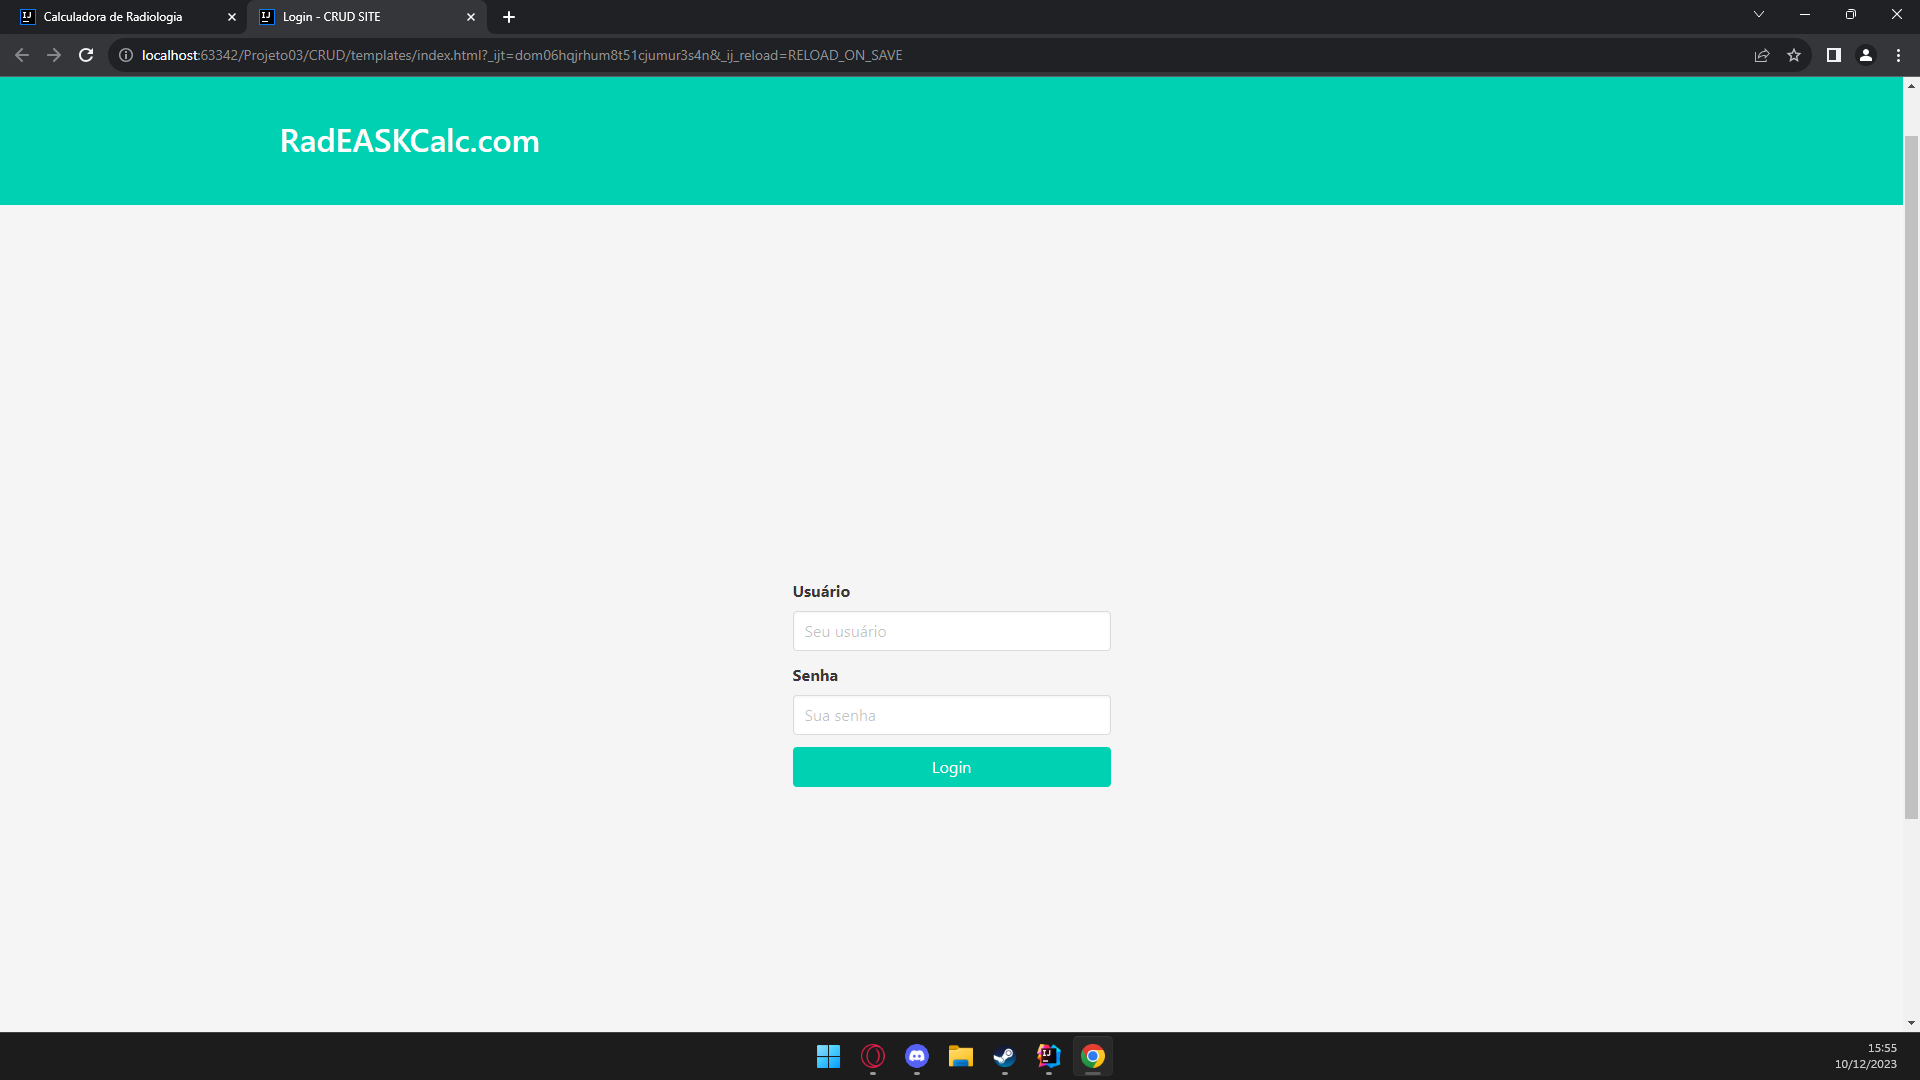
\includegraphics[width=0.9\columnwidth]{login.png}
  \caption{Login do site.}
  \label{fig:login}
\end{figure}

A Calculadora de Radiologia representa um avanço significativo na simplificação do processo de configuração de parâmetros radiológicos, desempenhando um papel crucial na obtenção de imagens de alta qualidade. Com uma interface intuitiva e configurações dinâmicas, esta ferramenta inovadora oferece a possibilidade de otimizar efetivamente o tempo dos profissionais de radiologia, resultando em diagnósticos mais precisos.

Além disso, destacamos que foi implementada uma tela de login dedicada no sistema. Essa funcionalidade permite que os usuários cadastrem-se e acessem a plataforma de forma segura. Agora, profissionais e clientes podem desfrutar de uma experiência mais personalizada e integrada, ampliando as possibilidades de interação e utilização da Calculadora de Radiologia.

\begin{figure}[h]
  \centering
  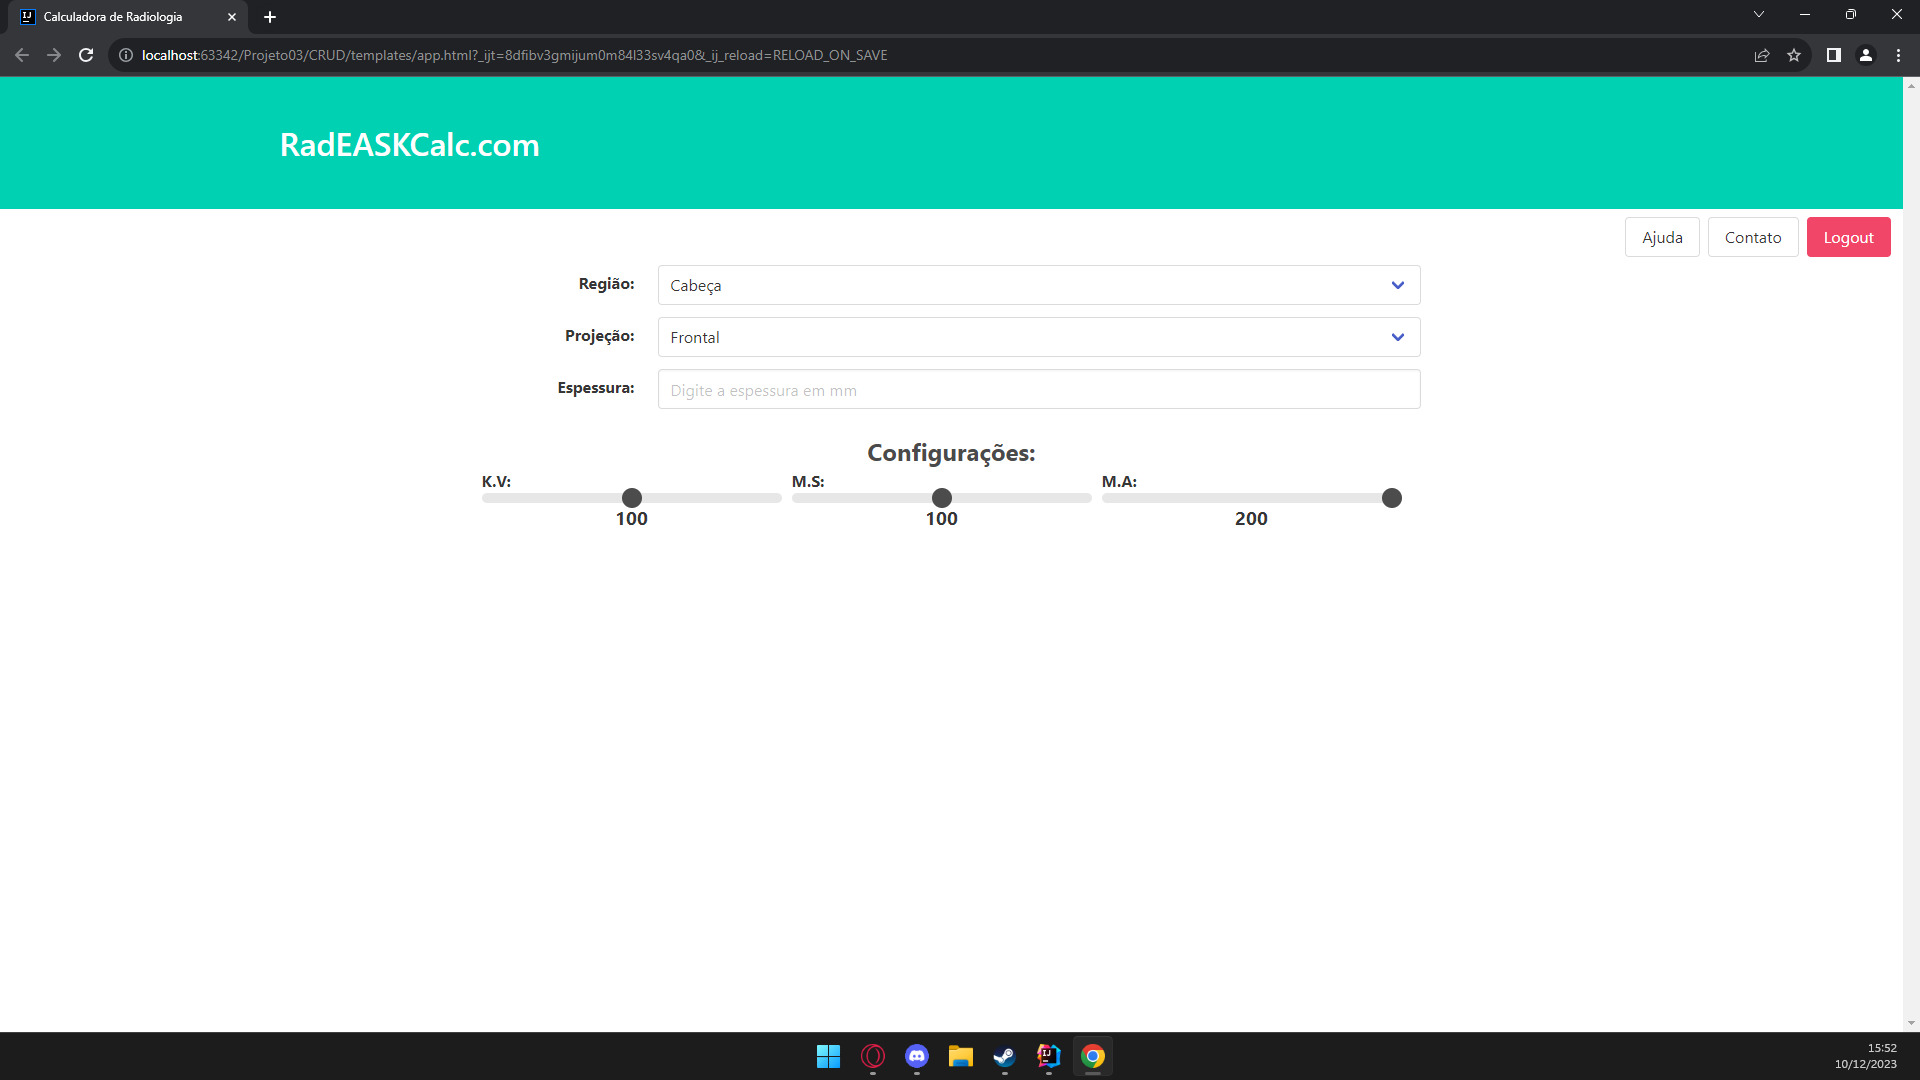
\includegraphics[width=0.9\columnwidth]{app.png}
  \caption{Calculadora no site.}
  \label{fig:calculadora}
\end{figure}

\begin{figure}[h]
  \centering
  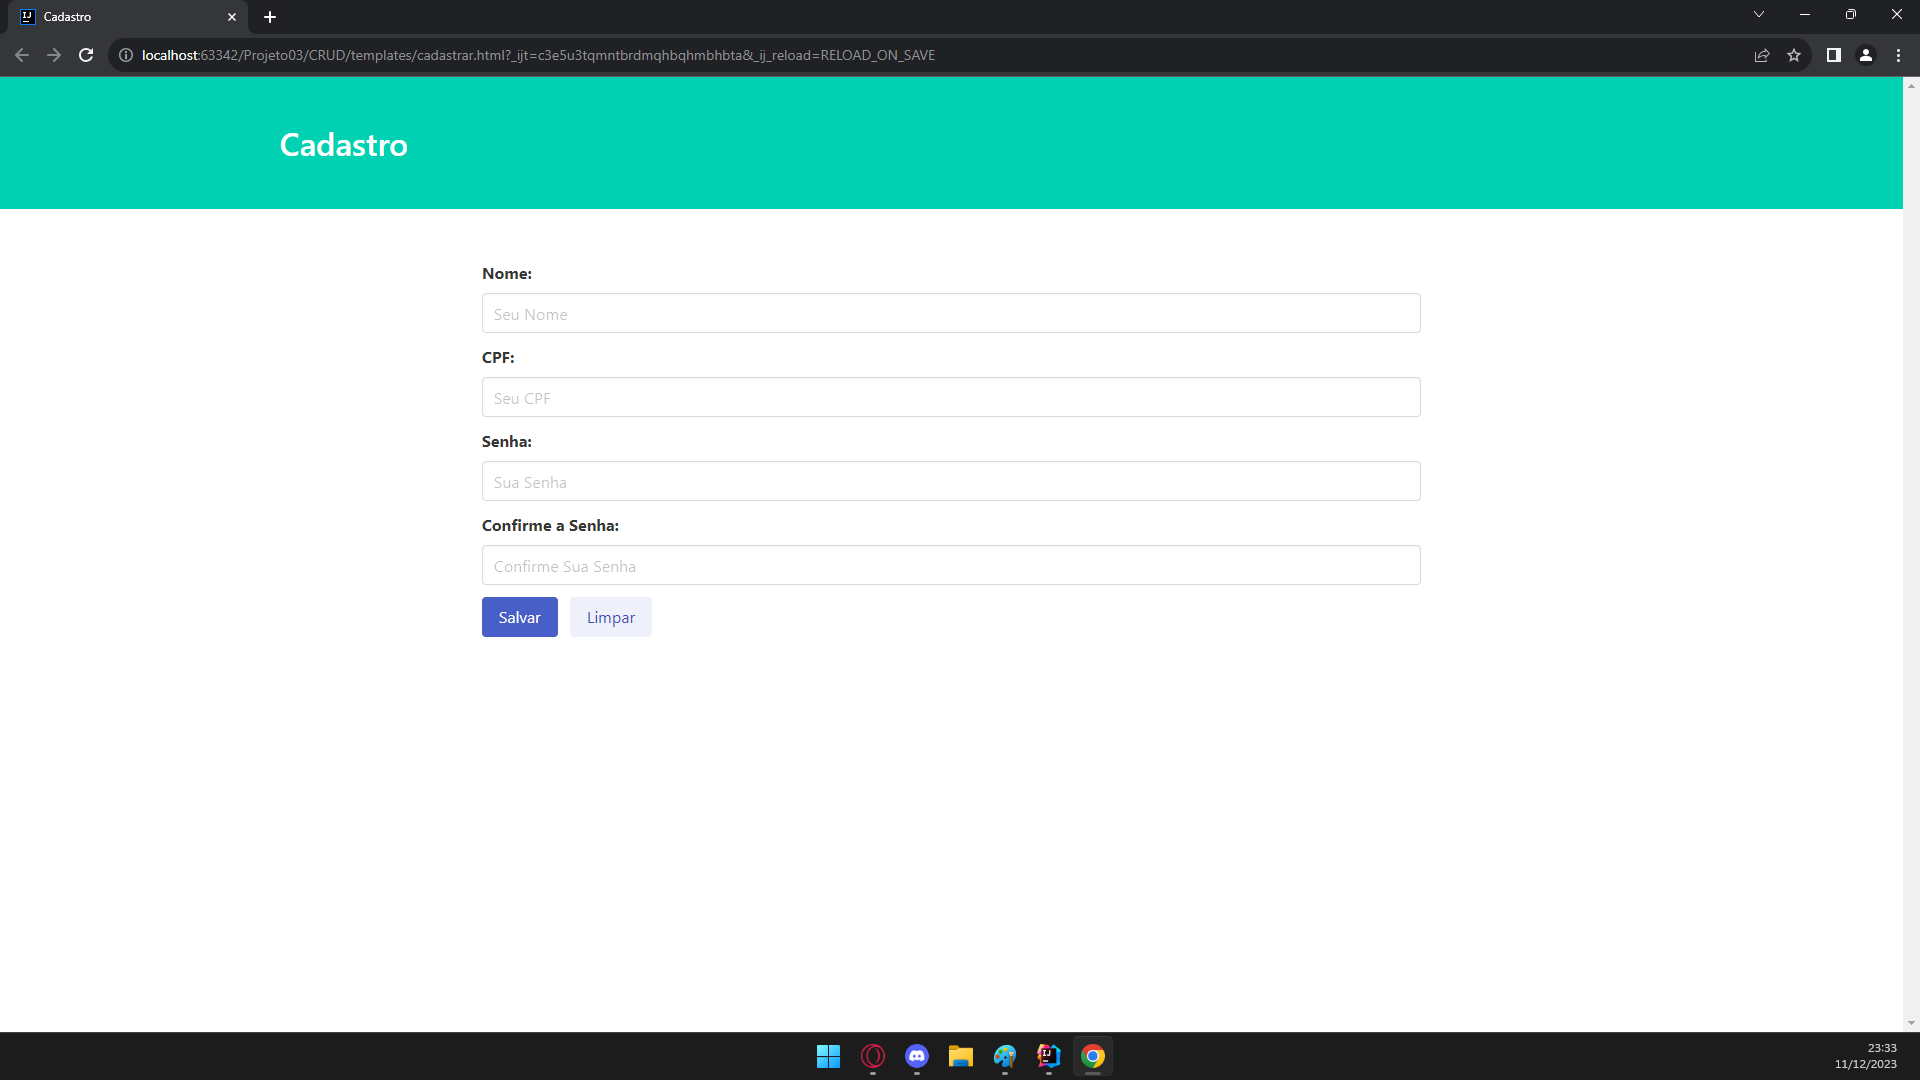
\includegraphics[width=0.9\columnwidth]{cadastro.png}
  \caption{Cadastro no site.}
  \label{fig:cadastro}
\end{figure}
 
\section{Conclusão}
A criação e implementação da Calculadora de Radiologia representam um marco significativo na busca pela otimização e aprimoramento dos processos radiológicos. Ao integrar tecnologias modernas, como HTML, CSS, JavaScript, o framework Bulma e o banco de dados MySQL, conseguimos desenvolver uma ferramenta abrangente e inovadora.

A interface intuitiva, as funcionalidades avançadas, e a capacidade de registro e autenticação de usuários demonstram o compromisso em oferecer uma experiência completa e segura aos profissionais de radiologia e clientes. A implementação bem-sucedida do banco de dados MySQL fortalece a eficiência na gestão e armazenamento de dados, contribuindo para uma análise precisa e confiável.

Os próximos passos visam expandir ainda mais a utilidade da Calculadora de Radiologia, registrando outras máquinas para melhorar a precisão dos cálculos, além de garantir atualizações contínuas para acompanhar as demandas da área radiológica.

Em conclusão, a Calculadora de Radiologia não apenas simplifica processos, mas também promove avanços essenciais na busca pela excelência em diagnósticos radiológicos. Este projeto representa um compromisso constante com a inovação, fornecendo uma solução robusta e adaptável às necessidades em constante evolução da medicina radiológica.

\section{Próximos Passos}
Diante do sucesso inicial da Calculadora de Radiologia, os próximos passos visam a expansão e aprimoramento contínuo do sistema. Entre as iniciativas planejadas, destaca-se o registro de novas máquinas radiológicas, permitindo uma precisão ainda maior nos cálculos, conforme ajustes específicos de cada modelo.
Umas das prioridades será o Registro Automático no Banco de Dados:} Após realizar os cálculos, a aplicação registra automaticamente as informações relevantes no banco de dados, garantindo uma gestão eficiente e segura das análises realizadas.

Além disso, está prevista a implementação de atualizações recorrentes, incorporando avanços tecnológicos, feedbacks dos usuários e aprimoramentos nas funcionalidades existentes. Essa abordagem assegura que a Calculadora de Radiologia permaneça na vanguarda das soluções tecnológicas na área radiológica, oferecendo sempre um serviço atualizado e eficiente.

\section*{Ambiente de Desenvolvimento}
Este projeto foi desenvolvido utilizando o ambiente de desenvolvimento IntelliJ IDEA. O IntelliJ IDEA é uma poderosa IDE (Integrated Development Environment) que oferece suporte abrangente para desenvolvimento em diversas linguagens, incluindo Java, HTML, CSS, JavaScript, entre outras.

\section{Referências}
https://www.jetbrains.com/idea/

https://www.oracle.com/br/mysql/

https://docs.spring.io/spring-framework/reference/overview.html

«MySQL :: MySQL 8.0 Release Notes :: Changes in MySQL 8.0.21 (2020-07-13, General Availability)». dev.mysql.com. 13 de julho de 2020. Consultado em 26 de setembro de 2020

https://docs.spring.io/spring-framework/reference/overview.html

Princípios de Radiologia Odontológica; Eric Whaites; 3º edição; ArtMed; 2002.
MORENO, José; SÁNCHEZ, Carlos (1985). Rayos X: Tomo I. Havana: Editorial pueblo y educacion.

Davydov, S.; Efimov, A. (Maio de 2005), IntelliJ IDEA. Professional'noe programmirovanie na Java (V podlinnike), ISBN 5-94157-607-2 1st ed. , BHV, p. 800, consultado em 17 de março de 2011, cópia arquivada em 9 de dezembro de 2013

https://spring.io/projects/spring-data-jpa

 "More deeply, the framework exists to separate the representation of information from user interaction." The DCI Architecture: A New Vision of Object-Oriented Programming Arquivado em 29 de setembro de 2017, no Wayback Machine. – Trygve Reenskaug and James Coplien – 20 de março de 2009.
https://www.thymeleaf.org

https://bulma.io/documentation/

\end{document}
